\documentclass[a4paper,titlepage,11pt]{article}

\usepackage[top=2.54cm, bottom=2.54cm, left=2.54cm, right=2.54cm]{geometry}
\usepackage[utf8x]{inputenc}
\usepackage{hyperref}
\usepackage{graphicx}
\usepackage{fancyhdr}
\usepackage{lastpage}
\usepackage{soul}

\pagestyle{fancy}
\fancyhf{}
\renewcommand{\headrulewidth}{0pt}
\cfoot{ \thepage \hspace{1pt} of \pageref{LastPage} }

\begin{document}

\begin{titlepage}
  \begin{center}
    {\scshape \huge Truthful Emergencies \par}
    \vspace{1cm}

    {\scshape \LARGE Report \par}
    \vspace{1.5cm}

    {\scshape \Large Network and Computer Security \par}
    \vspace{0.5cm}

    {\Large Alameda \par}
    \vfill

    {\itshape \Large Group 11 \par}
    \vfill

    \begin{tabular}{l l l}
      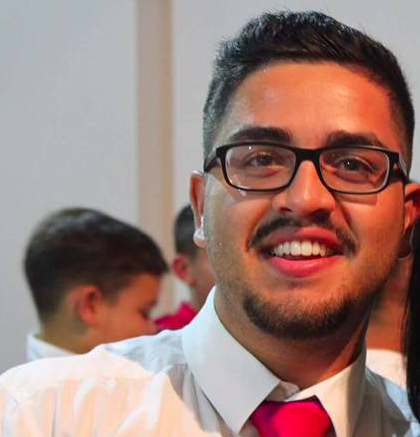
\includegraphics[width=20mm, height=20mm]{img/miguel.png} & Miguel Pinto & 79060\\
      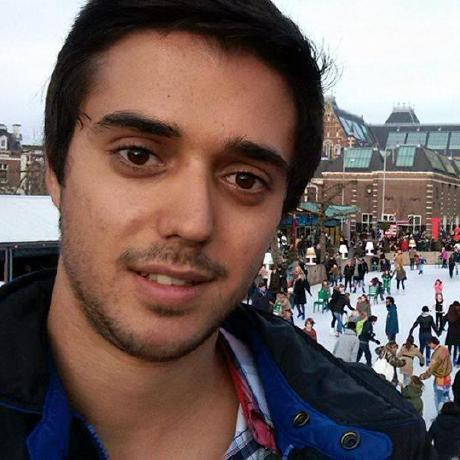
\includegraphics[width=20mm, height=20mm]{img/bernardo.jpeg} & Bernardo Casaleiro & 87827\\
      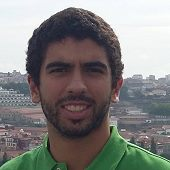
\includegraphics[width=20mm, height=20mm]{img/joao.jpeg} & João Godinho & 87830\\
    \end{tabular}
    \vfill

    {\large \today\par}
  \end{center}
\end{titlepage}

\section{Problem}
First response emergency systems are a limited resource. Their usage makes a difference in life-or-death situations!
Requesting an ambulance is a serious matter.
It should be simple, secure, fast and first of all always available.
For that the Dispatch Center must be fault tolerant.

It should separate the real requests from the false ones and provide a response accordingly.
Improper usage must be detected to avoid misallocation of resources while real requests should
trigger an appropriate response.

\section{Requirements}

\subsection{Application Requirements}
\begin{enumerate}
  \item Send an emergency request.
  \item Inform the estimated time for the user's request to be answered.
  \item \st{Confirm or deny if there is an emergency nearby.}
\end{enumerate}

\subsection{Server Requirements}
\begin{enumerate}
  \item Receive a request
  \item Insert a request in a queue depending on the user rating.
  \item \st{Request confirmation from users nearby the emergency.}
  \item Log the requests.
  \item Send the expected response time.
  \item Send the confirmation that an ambulance is on route.
  \item Rate the user accordingly at the end of the request.
  \item Temporarily block a user for abusive usage.
\end{enumerate}

\subsection{Security Requirements}
\begin{enumerate}
  \item Non-repudiation.
  \item \st{Fault tolerance to DoS.}
  \item \st{Firewall, responsible for filtering the requests.}
  \item \underline{Filter, responsible for filtering the requests.}
  \item Auditing mechanisms.
  \item Secure channel to communicate.
\end{enumerate}

\newpage

\section{Solution}
\subsection{Basic solution}
The main goal of this sprint is to build the foundation and the architecture to facilitate the implementation
of the security parts. There are no keys or certificates involved in this step so non-repudiation will not be
our goal here.

We will have a centralized Dispatch Central that will receive all the requests from the Users.

Auditing mechanisms will be considered in this phase and for that we will use logs on the Central side.

After processing the request, and approving it, the Dispatch sends the confirmation message that an ambulance is
on the way. Otherwise the user will be accounted for the incorrect usage and warned of the possible consequences
of further reckless behavior.

After attending the emergency the team sent provides feedback regarding the truthfulness of the emergency.

The user will be registered into a database with a ranking associated that will be used for the placement in queue.

\subsection{Intermediate solution}
In this phase, we will create manually all the keys and certificates\footnote{self-signed}.

Each entity will have his own set of keys, but the certificates will have to be requested to the CA to obtain
the public key.

Each message sent by the user will be signed with his own private key.

The Dispatch Central will retrieve the user public key from the certificate that was requested after receiving
the message and then deciphers it. The procedure is the same for the message flow from the Dispatch to the user.

In this phase we will also build a network level firewall, with some basic rules to discard duplicate packets
and redirect connections to secure ports (HTTPS).

\subsection{Advanced solution}
On this last phase of the project, we will focus on fault tolerance on the primary server (DoS, crash, etc.).
We will also focus in updating the firewall to an intrusion detection system. This IDS will receive the data
from the sensors of the phone and analize its content to verify the veracity of the message.


\section{Results}
Our solution has two main components: the dispatch central and the user aplication.
In order to meet the security requirements we also implemented a certificate authority and a confirmation central.

The user aplication allow the user to send emergency requests. When starting the application it first sends
the user certificate to the certificate authority. Then the user is able to send requests to the dispatch central.

When receiving a request the dispatch central asks the CA for the user certificate in order to decipher the request and
passes it through a series of filters to exclude false ones. Only processing the accepted ones. The dispatch central then
notifies the user either that help is on the way or that the request sent was false and reminds the user of the consequences.
After an emergency team is dispatched the server asks the confirmation central to rate the request depending on the
authenticity of the emergency, awarding or penalizing the user.

All this comunications between the components are made using Java SSL Sockets in order to guarantee a secure channels and
always cyphered using the proper certificates provided by the certificate authority.

\begin{figure}[ht]
    \centering
    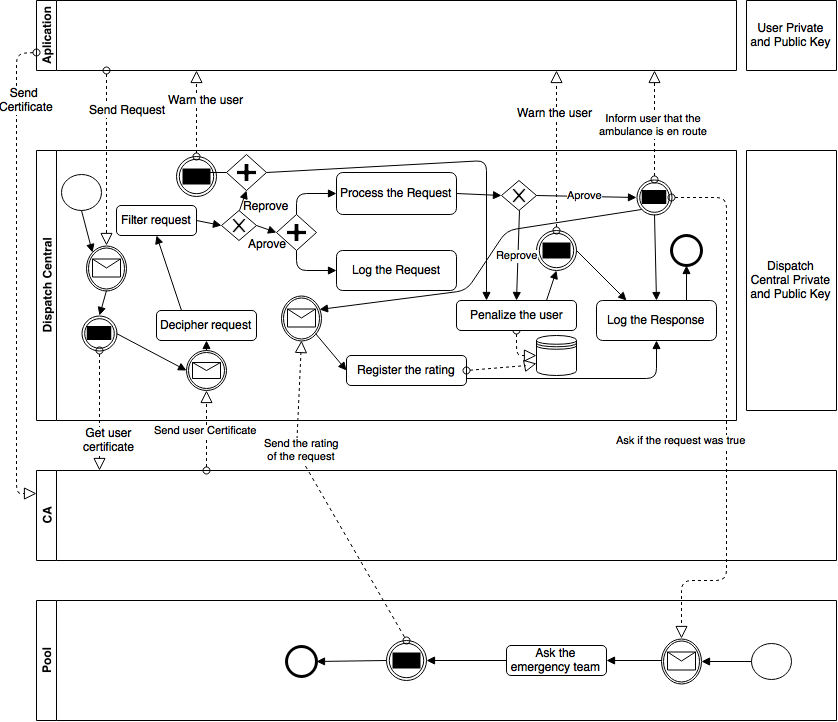
\includegraphics[scale=0.45]{img/advanced-solution.png}
\end{figure}

\section{Evaluation}
With our implementation we reached the majority of the security requirements proposed. As well as the majority of the
functional requirements.

We began by aproaching the \textbf{Auditing Mechanisms} point using the Log4j api to keep a record of every request received and
action taken. Moving then to the \textbf{Secure Channel} point where we upgraded from Java Sockets to Java SSL Sockets, and to the
\textbf{Non-Repudiation} point using the certificates and a certificate authority to distribute them.

Our initial goal in order to filter the requests received was to build a firewall but due to the lack of time we opted for a
simpler solution and implemented a filter. This filter allow us to somewhat filter the invalid requests in the moment the server
receives and deciphers them.

Another point that we had to adapt was the \textbf{Fault Tolerance to DoS}. This initially was a really important point for us and we
hoped to distribute our system and use a load balance to optimize resource use and avoid overload of a single resource. But with the
project's development and the scarce time we decided that it was just not possible.

We also hoped to move from a terminal that simulates a user application to an actual Android application where we would have access to
the user location and implement new features like \textit{confimation of a nearby request based on the user location}. Although our
expectations it had to be put aside.

\section{Conclusion}

\section{References}

\subsection{Tool References}
\begin{description}
  \item [PostgreSQL] \href{https://www.postgresql.org}{Database to save the users.}
  \item [javax.net.ssl.SSLServerSocket] \href{https://docs.oracle.com/javase/7/docs/api/java/net/Socket.html}{Establish a secure connection.}
  \item [PostgreSQL JDBC] \href{https://jdbc.postgresql.org}{Driver to use PostgreSQL with Java.}
  \item [Log4j] \href{http://logging.apache.org/log4j/2.x/}{Logging system.}
\end{description}

\end{document}
